\documentclass[conference,compsoc]{IEEEtran}
\usepackage{datetime}
\usepackage{caption}
\usepackage{listings}
\usepackage{graphicx}

\lstdefinestyle{mystyle}{
    basicstyle=\small\sffamily,
	numbers=left,
	numberstyle=\tiny,
	frame=tb,
	breakatwhitespace=true,  
    	breaklines=true,
	columns=fullflexible,
	showstringspaces=false}



% *** CITATION PACKAGES ***
%
\ifCLASSOPTIONcompsoc
  % IEEE Computer Society needs nocompress option
  % requires cite.sty v4.0 or later (November 2003)
  \usepackage[nocompress]{cite}
\else  
  % normal IEEE
  \usepackage{cite} 
\fi 
% cite.sty was written by Donald Arseneau
% V1.6 and later of IEEEtran pre-defines the format of the cite.sty package
% \cite{} output to follow that of the IEEE. Loading the cite package will
% result in citation numbers being automatically sorted and properly
% "compressed/ranged". e.g., [1], [9], [2], [7], [5], [6] without using
% cite.sty will become [1], [2], [5]--[7], [9] using cite.sty. cite.sty's
% \cite will automatically add leading space, if needed. Use cite.sty's
% noadjust option (cite.sty V3.8 and later) if you want to turn this off
% such as if a citation ever needs to be enclosed in parenthesis.
% cite.sty is already installed on most LaTeX systems. Be sure and use
% version 5.0 (2009-03-20) and later if using hyperref.sty.
% The latest version can be obtained at:
% http://www.ctan.org/pkg/cite
% The documentation is contained in the cite.sty file itself.
%
% Note that some packages require special options to format as the Computer
% Society requires. In particular, Computer Society  papers do not use
% compressed citation ranges as is done in typical IEEE papers
% (e.g., [1]-[4]). Instead, they list every citation separately in order
% (e.g., [1], [2], [3], [4]). To get the latter we need to load the cite
% package with the nocompress option which is supported by cite.sty v4.0
% and later.

% *** GRAPHICS RELATED PACKAGES ***
%
\ifCLASSINFOpdf
  % \usepackage[pdftex]{graphicx}
  % declare the path(s) where your graphic files are
  % \graphicspath{{../pdf/}{../jpeg/}}
  % and their extensions so you won't have to specify these with
  % every instance of \includegraphics
  % \DeclareGraphicsExtensions{.pdf,.jpeg,.png}
\else
  % or other class option (dvipsone, dvipdf, if not using dvips). graphicx
  % will default to the driver specified in the system graphics.cfg if no
  % driver is specified.
  % \usepackage[dvips]{graphicx}
  % declare the path(s) where your graphic files are
  % \graphicspath{{../eps/}}
  % and their extensions so you won't have to specify these with
  % every instance of \includegraphics
  % \DeclareGraphicsExtensions{.eps}
\fi
% graphicx was written by David Carlisle and Sebastian Rahtz. It is
% required if you want graphics, photos, etc. graphicx.sty is already
% installed on most LaTeX systems. The latest version and documentation
% can be obtained at: 
% http://www.ctan.org/pkg/graphicx
% Another good source of documentation is "Using Imported Graphics in
% LaTeX2e" by Keith Reckdahl which can be found at:
% http://www.ctan.org/pkg/epslatex
%
% latex, and pdflatex in dvi mode, support graphics in encapsulated
% postscript (.eps) format. pdflatex in pdf mode supports graphics
% in .pdf, .jpeg, .png and .mps (metapost) formats. Users should ensure
% that all non-photo figures use a vector format (.eps, .pdf, .mps) and
% not a bitmapped formats (.jpeg, .png). The IEEE frowns on bitmapped formats
% which can result in "jaggedy"/blurry rendering of lines and letters as
% well as large increases in file sizes.
%
% You can find documentation about the pdfTeX application at:
% http://www.tug.org/applications/pdftex


% *** MATH PACKAGES ***
%
%\usepackage{amsmath}
% A popular package from the American Mathematical Society that provides
% many useful and powerful commands for dealing with mathematics.
%
% Note that the amsmath package sets \interdisplaylinepenalty to 10000
% thus preventing page breaks from occurring within multiline equations. Use:
%\interdisplaylinepenalty=2500
% after loading amsmath to restore such page breaks as IEEEtran.cls normally
% does. amsmath.sty is already installed on most LaTeX systems. The latest
% version and documentation can be obtained at:
% http://www.ctan.org/pkg/amsmath

% *** SPECIALIZED LIST PACKAGES ***
%
%\usepackage{algorithmic}
% algorithmic.sty was written by Peter Williams and Rogerio Brito.
% This package provides an algorithmic environment fo describing algorithms.
% You can use the algorithmic environment in-text or within a figure
% environment to provide for a floating algorithm. Do NOT use the algorithm
% floating environment provided by algorithm.sty (by the same authors) or
% algorithm2e.sty (by Christophe Fiorio) as the IEEE does not use dedicated
% algorithm float types and packages that provide these will not provide
% correct IEEE style captions. The latest version and documentation of
% algorithmic.sty can be obtained at:
% http://www.ctan.org/pkg/algorithms
% Also of interest may be the (relatively newer and more customizable)
% algorithmicx.sty package by Szasz Janos:
% http://www.ctan.org/pkg/algorithmicx


% *** ALIGNMENT PACKAGES ***
%
%\usepackage{array}
% Frank Mittelbach's and David Carlisle's array.sty patches and improves
% the standard LaTeX2e array and tabular environments to provide better
% appearance and additional user controls. As the default LaTeX2e table
% generation code is lacking to the point of almost being broken with
% respect to the quality of the end results, all users are strongly
% advised to use an enhanced (at the very least that provided by array.sty)
% set of table tools. array.sty is already installed on most systems. The
% latest version and documentation can be obtained at:
% http://www.ctan.org/pkg/array

% IEEEtran contains the IEEEeqnarray family of commands that can be used to
% generate multiline equations as well as matrices, tables, etc., of high
% quality.

% *** SUBFIGURE PACKAGES ***
%\ifCLASSOPTIONcompsoc
%  \usepackage[caption=false,font=footnotesize,labelfont=sf,textfont=sf]{subfig}
%\else
%  \usepackage[caption=false,font=footnotesize]{subfig}
%\fi
% subfig.sty, written by Steven Douglas Cochran, is the modern replacement
% for subfigure.sty, the latter of which is no longer maintained and is
% incompatible with some LaTeX packages including fixltx2e. However,
% subfig.sty requires and automatically loads Axel Sommerfeldt's caption.sty
% which will override IEEEtran.cls' handling of captions and this will result
% in non-IEEE style figure/table captions. To prevent this problem, be sure
% and invoke subfig.sty's "caption=false" package option (available since
% subfig.sty version 1.3, 2005/06/28) as this is will preserve IEEEtran.cls
% handling of captions.
% Note that the Computer Society format requires a sans serif font rather
% than the serif font used in traditional IEEE formatting and thus the need
% to invoke different subfig.sty package options depending on whether
% compsoc mode has been enabled.
%
% The latest version and documentation of subfig.sty can be obtained at:
% http://www.ctan.org/pkg/subfig

% *** FLOAT PACKAGES ***
%
%\usepackage{fixltx2e}
% fixltx2e, the successor to the earlier fix2col.sty, was written by
% Frank Mittelbach and David Carlisle. This package corrects a few problems
% in the LaTeX2e kernel, the most notable of which is that in current
% LaTeX2e releases, the ordering of single and double column floats is not
% guaranteed to be preserved. Thus, an unpatched LaTeX2e can allow a
% single column figure to be placed prior to an earlier double column
% figure.
% Be aware that LaTeX2e kernels dated 2015 and later have fixltx2e.sty's
% corrections already built into the system in which case a warning will
% be issued if an attempt is made to load fixltx2e.sty as it is no longer
% needed.
% The latest version and documentation can be found at:
% http://www.ctan.org/pkg/fixltx2e

%\usepackage{stfloats}
% stfloats.sty was written by Sigitas Tolusis. This package gives LaTeX2e
% the ability to do double column floats at the bottom of the page as well
% as the top. (e.g., "\begin{figure*}[!b]" is not normally possible in
% LaTeX2e). It also provides a command:
%\fnbelowfloat
% to enable the placement of footnotes below bottom floats (the standard
% LaTeX2e kernel puts them above bottom floats). This is an invasive package
% which rewrites many portions of the LaTeX2e float routines. It may not work
% with other packages that modify the LaTeX2e float routines. The latest
% version and documentation can be obtained at:
% http://www.ctan.org/pkg/stfloats
% Do not use the stfloats baselinefloat ability as the IEEE does not allow
% \baselineskip to stretch. Authors submitting work to the IEEE should note
% that the IEEE rarely uses double column equations and that authors should try
% to avoid such use. Do not be tempted to use the cuted.sty or midfloat.sty
% packages (also by Sigitas Tolusis) as the IEEE does not format its papers in
% such ways.
% Do not attempt to use stfloats with fixltx2e as they are incompatible.
% Instead, use Morten Hogholm'a dblfloatfix which combines the features
% of both fixltx2e and stfloats:
%
% \usepackage{dblfloatfix}
% The latest version can be found at:
% http://www.ctan.org/pkg/dblfloatfix

% *** PDF, URL AND HYPERLINK PACKAGES ***
%
%\usepackage{url}
% url.sty was written by Donald Arseneau. It provides better support for
% handling and breaking URLs. url.sty is already installed on most LaTeX
% systems. The latest version and documentation can be obtained at:
% http://www.ctan.org/pkg/url
% Basically, \url{my_url_here}.

% *** Do not adjust lengths that control margins, column widths, etc. ***
% *** Do not use packages that alter fonts (such as pslatex).         ***
% There should be no need to do such things with IEEEtran.cls V1.6 and later.
% (Unless specifically asked to do so by the journal or conference you plan
% to submit to, of course. )

% correct bad hyphenation here
\hyphenation{op-tical net-works semi-conduc-tor}
   
\usepackage{hyperref}
 
\begin{document}
\lstset{style=mystyle}
% 
% paper title
% Titles are generally capitalized except for words such as a, an, and, as,
% at, but, by, for, in, nor, of, on, or, the, to and up, which are usually
% not capitalized unless they are the first or last word of the title.
% Linebreaks \\ can be used within to get better formatting as desired.
% Do not put math or special symbols in the title.
\title{BSP Project Description:\\
OrbitCalc - A simplified version of the solar system\\
{\small \today~-~\currenttime}}

 
% author names and affiliations
% use a multiple column layout for up to three different
% affiliations
\author{\IEEEauthorblockN{Henrik Klasen}
\IEEEauthorblockA{University of Luxembourg\\
Email: henrik.klasen.001@student.uni.lu}
\\
{\bf This report has been produced under the supervision of:}\\
\IEEEauthorblockN{Gabriel Garcia}
\IEEEauthorblockA{University of Luxembourg\\
Email: gabriel.garcia@uni.lu}%
}

% conference papers do not typically use \thanks and this command
% is locked out in conference mode. If really needed, such as for
% the acknowledgment of grants, issue a \IEEEoverridecommandlockouts
% after \documentclass

% for over three affiliations, or if they all won't fit within the width
% of the page (and note that there is less available width in this regard for
% compsoc conferences compared to traditional conferences), use this
% alternative format:
% 
%\author{\IEEEauthorblockN{Michael Shell\IEEEauthorrefmark{1},
%Homer Simpson\IEEEauthorrefmark{2},
%James Kirk\IEEEauthorrefmark{3}, 
%Montgomery Scott\IEEEauthorrefmark{3} and
%Eldon Tyrell\IEEEauthorrefmark{4}}
%\IEEEauthorblockA{\IEEEauthorrefmark{1}School of Electrical and Computer Engineering\\
%Georgia Institute of Technology,
%Atlanta, Georgia 30332--0250\\ Email: see http://www.michaelshell.org/contact.html}
%\IEEEauthorblockA{\IEEEauthorrefmark{2}Twentieth Century Fox, Springfield, USA\\
%Email: homer@thesimpsons.com}
%\IEEEauthorblockA{\IEEEauthorrefmark{3}Starfleet Academy, San Francisco, California 96678-2391\\
%Telephone: (800) 555--1212, Fax: (888) 555--1212}
%\IEEEauthorblockA{\IEEEauthorrefmark{4}Tyrell Inc., 123 Replicant Street, Los Angeles, California 90210--4321}}




% use for special paper notices
%\IEEEspecialpapernotice{(Invited Paper)}




% make the title area
\maketitle

%to remove for your report
%\footnote{}

% As a general rule, do not put math, special symbols or citations
% in the abstract
\begin{abstract}
With scientific endeavours becoming more cost intensive, there is a need to plan specific missions into minor details. For having the means to plan such missions, for example to the edge of the solar system, to the depth of the oceans and onto the surface of other celestial bodies, there has to be a computational model, which virtually has any property, any side factor and any physical property of the environment the mission planners expect to encounter. The development of one such computational model with a potential use case in space exploration is the topic of this Bachelor Semester Project. 
%\\ (100 words) \\ In total 1225 words, ca. 65\%
%This document is a template for the project subject description  (PSD for short) report that is to be delivered by any BiCS student at the end of the phase 1 of a Bachelor Semester Project (BSP). The Latex source files are available at:\\
%\href{https://github.com/nicolasguelfi/lu.uni.course.bics.global}{{\underline{\textbf{https://github.com/nicolasguelfi/lu.uni.course.bics.global}}}}\\
  
%This template is to be used using the Latex document preparation system or using any document preparation system. The whole document should be 1500 words ($\pm$ 500 words) for S2 to S6 students and 3000 words ($\pm$ 500 words) for S1 students (excluding the annexes) and the proportions must be preserved. The other documents to be delivered (summaries, \ldots) should have their format adapted from this template.\\

%A tutor (or any person having contributed to the BSP work) is not a co-author per se for a student's work. It is possible to exploit a BSP report to produce a scientific and technical publication. In this case, the authors list has to be discussed and agreed with the concerned parties.

\end{abstract}

% no keywords

% For peer review papers, you can put extra information on the cover
% page as needed:
% \ifCLASSOPTIONpeerreview
% \begin{center} \bfseries EDICS Category: 3-BBND \end{center}
% \fi
%
% For peerreview papers, this IEEEtran command inserts a page break and
% creates the second title. It will be ignored for other modes.
\IEEEpeerreviewmaketitle






% \subsection{Constraints}
% Provide all the constraints that were to be considered for the project.
% A constraint is a property that is agreed by you and your PAT to have been satisfied before starting the project.
% An example could be ``good level in Python programming''. 
% As a consequence the work done to satisfy the constraints cannot be presented as a deliverable of the BSP.

\section{Main required competencies } 
%(107/100-200 words  5.35\%)
%Describe in these sections the main scientific and technical competencies that is required to be known by you before starting the project.
%Do not describe in details this knowledge but only abstractly. All the content of this section shall not be used, even partially, in the deliverable sections.
%It is important not to include in this section all the knowledge you have been obliged to acquire in order to produce the deliverable. It should only state the knowledge the student possessed before starting the project and that was mandatory to possess to be capable to produce the deliverables. It explicitly defines  the technical and scientific pre-condition for the project. It is also useful to avoid project failures due to over or under complex subjects.


\subsection{Scientific main required competencies }
%(44 words)
Before starting the Bachelor Semester Project, the student had some experience in orbital mechanics, which includes the basics of (gravitational) force vectors. \\
Next to that, the student had some experience in constructing mathematical and physical models with certain simplifications for computational ease.
\subsection{Technical main required competencies }
%(63 words)
As the technical deliverable is about the implementation of a basic solar system simulation in Unity, the student already knows how to work with Unitys' scaling, transformation and rotation system and their script application programming interfaces (APIs) in C\#. Also the basics of game and simulation development are known, as it was part of a small course in the Computer Science Summer Camp at Hochschule Trier.

\section{ A computational model for a solar system simulation }
%(704/800 words)
The scientific part of this Bachelor Semester Project is about modelling a suitable, simplified model of the solar system.\\
It will consist of three parts. The first part being about the fundamentals of computational modelling, which will take a look at the approach of breaking real world data down to a computable model. This model can be emulated by a computer program.\\
As the title of this Bachelor Semester Project implies, the second part of the scientific part is about modelling a model with some constraints and simplifications. This model will include the basics of orbital mechanics, as well as the fundamental concepts of Newtonian physics.\\ 
The domains of this project are:
\begin{itemize}
	\item \emph{Computational Modelling}: This domain is all about breaking down real life environments and behaviours into equations and algorithms for simulating the environment as good as possible with certain simplifications.
	\item \emph{Simulations}: Simulations are a computational approach to emulate real life behaviours of objects and environments on computers. They are used for example for optimizing the trajectories in space, simulating fluid dynamics or aerodynamics for optimizing the fuel efficiency of cars.
	\item \emph{Scientific Computing}: Scientific Computing is an interdisciplinary discipline bound to develop approaches for algorithms, models and software. These are used for simulating real world behaviour as close as possible. This means, that computational modelling and simulations are both a subset of scientific computing, which is the broader scientific topic. 
\end{itemize}
The scientific part will tackle the following scientific question: \emph{How can scientists model a simplified simulation of the solar system?} \\
To find a satisfying answer to this question, it is necessary to answer the related questions:
\begin{itemize}
	\item \emph{What is a computational model?}: This question aims on answering the most basic and fundamental question of this project. The results of this question are required to later on build and model the computational model.
	\item \emph{What environmental factors of the solar system have to be considered?}: This question aims on answering, \emph{how} the model will look like. This includes the examination of the utilized simplifications, methodologies and an analysis of the factors influencing the selection of specific approaches.
	\item \emph{How can the model be modelled? }: With this question, the goal is to find equations and algorithms that facilitate an accurate representation of the computational model. This part is meant to include all the orbital mechanics theory needed. 
\end{itemize}
As the goal is to find satisfying answers to the questions above, a state-of-the-art study will be conducted. 
Based on this study, the subsequent resources are used to address the scientific question:
\begin{itemize}
	\item \cite{PhysicsSimulationsLargeWorlds}: This publication is about the computational cost of large scale physics simulations. It will mainly be used in the section for the question "\emph{What environmental factors of the solar system have to be considered?}", as it is about modelling the computational model itself. 
	\item \cite{ComputationalModelling}: The main point in using this publication is to find out a way to properly model a computational model. It provides many examples for computational models for several different simulations, which might help when modelling the solar system later in the project.
	\item \cite{ScientificComputing}: This resource is about scientific computing. As its objective is to teach undergraduate students the fundamentals of scientific computing and numerical methods to model a simulation or whichever model needed, it is well suitable for this Bachelor Semester Project. It will be used for getting some insights on how scientific computing is used today and how it \emph{can} be used in this project.
\end{itemize}

With the use of these resources, the scientific part will focus on delivering the most useful and crucial information to develop a satisfying model of the solar system. The results of this part will later on be used in the technical part of this bachelor semester project, which is all about the implementation of a three dimensional solar system in Unity. In the last section of this part of the project, we will take a look at which factors cannot be simulated in the model developed and which parts could possibly be added in future extensions, but which exceed the scope of this project. \\
The overall goal of this deliverable is to ensure, that the reader can understand the design decisions in the technical part. The results of this section will be used as a fundamental basis of the technical deliverable and the implementation.

% Technical deliverable from here on!

\section{ Implementation of a virtual solar system }
%(710/800 words)
The technical part of this Bachelor Semester Project is about the implementation of the computational model developed in the scientific part. In fact, it is about the implementation of a virtual version of the solar system. \\
While the scientific part is more about the "\emph{What do we want to simulate?}", this part is more about the "\emph{How do we implement what we want to simulate?}". The goal with this deliverable is, to get to know how to implement scientific computing models in a given environment. \\
The domains of this deliverable are:
\begin{itemize}
	\item \emph{Unity}: A state of the art game engine for three dimensional and two dimensional games. With its powerful, built-in physics engine, it is able to also create realistic simulations, such as digital twinning, fluid simulations, as well as large field gravitational simulations, which is the goal in this project.
	\item \emph{Visual Studio}: A powerful code editor for all of the programming languages in the .NET Framework. This IDE has Unity integration, which simplifies the development of programs in Unity by a lot. 
	\item \emph{C\#}: A language in the .NET framework, which was heavily influenced by C++ and Java. It is object-oriented and Unity provides an API to its editor to this language. 
\end{itemize} 
As for the technical deliverable, there is not as much literature such as official scientific papers or publications. The main source of information will be the scientific deliverable, e.g. for the equations describing the gravitational law. Next to that, the official Unity Documentation (linked in \cite{UnityDoc}) will be used for any further documentation regarding Unitys API. \\ 
The technical deliverable will provide some key features:
\begin{itemize}
	\item \emph{Gravity}: According to the Newtonian gravitational law. Further details will be in the scientific part of the report.
	\item \emph{Real scale}: The scale of the objects in the solar system will correspond to their actual scale in the real solar system. This will (hopefully) ensure a higher degree of realism and ease gravitational calculations, which are based on the distances.
	\item \emph{Realistic lighting}: As the sun is more or less the only high intensity light source in the solar system, the simulation will use a point light source which will shine light from the suns position. 
	\item \emph{User controllable Satellite}: This will help the user experience navigating a satellite in a three dimensional solar system with objects influencing the trajectory of the space probe.
\end{itemize}

The program will eventually include a Graphical User Interface, for which some parameters are needed. So far it is planned to include the parameters for two objects, mainly x-y-z position of the objects. It is also task of this part to find out, which data is going to be displayed in a light-weight interface, which provides the user enough information for controlling satellite and camera. For example, the data, currently planned to be displayed are: 
\begin{itemize}
	\item Velocity of user controlled camera: To measure how fast the user is going in the solar system
	\item Velocity of the satellite: To enable the user to calculate where the space probe will be when.
	\item Distance of the satellite to the sun: To locate the position of the satellite
	\item Coordinates of the satellite: Locate the satellite in a three-dimensional space
	\item Coordinates of the camera: Locate the user controlled camera in three-dimensional space
	\item Distance camera – Sun: To locate the camera on a relative basis in the solar system
	\item Labels of the planets: Locate the planets relative to the camera
	\item Planet orbit paths: Locate the orbits of the planets
	\item Satellite trajectory: Display the points, the satellite already passed to estimate the further trajectory
\end{itemize}

As the user will be able to control the camera, it will be required for this project, to map keys on the keyboard to certain movements, to enable the user to experience the virtual solar system. As of now, the keys are mapped as follows
\begin{itemize}
	\item W – Forwards movement relative to current rotation
	\item A – Left movement relative to current rotation
	\item S – Backwards movement relative to current rotation
	\item D – Right movement relative to current rotation
	\item X – Upwards movement relative to current rotation
	\item Y – Downwards movement relative to current rotation
	\item Arrow Key Left – Rotation Left (Z-Axis)
	\item Arrow Key Right – Rotation Right (Z-Axis)
	\item Arrow Key Up – Rotation Upwards (X-Axis)
	\item Arrow Key Down – Rotation Downwards (X-Axis)
\end{itemize}

Also the  satellite will be controllable by the user, to ensure, that the user gets a better understanding of the complexity of navigating in a three-dimensional space under the influence of gravitational pull to other celestial bodies. 


% An example of a floating figure using the graphicx package.
% Note that \label must occur AFTER (or within) \caption.
% For figures, \caption should occur after the \includegraphics.
% Note that IEEEtran v1.7 and later has special internal code that
% is designed to preserve the operation of \label within \caption
% even when the captionsoff option is in effect. However, because
% of issues like this, it may be the safest practice to put all your
% \label just after \caption rather than within \caption{}.
%
% Reminder: the "draftcls" or "draftclsnofoot", not "draft", class
% option should be used if it is desired that the figures are to be
% displayed while in draft mode.
%
%\begin{figure}[!t]
%\centering
%\includegraphics[width=2.5in]{myfigure}
% where an .eps filename suffix will be assumed under latex, 
% and a .pdf suffix will be assumed for pdflatex; or what has been declared
% via \DeclareGraphicsExtensions.
%\caption{Simulation results for the network.}
%\label{fig_sim}
%\end{figure}

% Note that the IEEE typically puts floats only at the top, even when this
% results in a large percentage of a column being occupied by floats.
\section{Plagiarism statement}

I declare that I am aware of the following facts:
\begin{itemize}
	\item As a student at the University of Luxembourg I must respect the rules of intellectual honesty, in particular not to resort to plagiarism, fraud or any other method that is illegal or contrary to scientific integrity.
	\item My report will be checked for plagiarism and if the plagiarism check is positive, an internal procedure will be started by my tutor. I am advised to request a pre-check by my tutor to avoid any issue.
	\item As declared in the assessment procedure of the University of Luxembourg, plagiarism is committed whenever the source of information used in an assignment, research report, paper or otherwise published/circulated piece of work is not properly acknowledged. In other words, plagiarism is the passing off as one’s own the words, ideas or work of another person, without attribution to the author. The omission of such proper acknowledgement amounts to claiming authorship for the work of another person. Plagiarism is committed regardless of the language of the original work used. Plagiarism can be deliberate or accidental.
	Instances of plagiarism include, but are not limited to:
	\begin{enumerate}
		\item Not putting quotation marks around a quote from another person’s work
		\item Pretending to paraphrase while in fact quoting
		\item Citing incorrectly or incompletely
		\item Failing to cite the source of a quoted or paraphrased work
		\item Copying/reproducing sections of another person’s work without acknowledging the source
		\item Paraphrasing another person’s work without acknowledging the source
		\item Having another person write/author a work for oneself and submitting/publishing it (with permission, with or without compensation) in one’s own name (‘ghost-writing’)
		\item Using another person’s unpublished work without attribution and permission (‘stealing’)
		\item Presenting a piece of work as one’s own that contains a high proportion of quoted/copied or paraphrased text (images, graphs, etc.), even if adequately referenced
	\end{enumerate}
	Auto- or self-plagiarism, that is the reproduction of (portions of a) text previously written by the author without citing that text, i.e. passing previously authored text as new, may be regarded as fraud if deemed sufficiently severe.
\end{itemize}

% An example of a double column floating figure using two subfigures.
% (The subfig.sty package must be loaded for this to work.)
% The subfigure \label commands are set within each subfloat command,
% and the \label for the overall figure must come after \caption.
% \hfil is used as a separator to get equal spacing.
% Watch out that the combined width of all the subfigures on a 
% line do not exceed the text width or a line break will occur.
%
%\begin{figure*}[!t]
%\centering
%\subfloat[Case I]{\includegraphics[width=2.5in]{box}%
%\label{fig_first_case}}
%\hfil
%\subfloat[Case II]{\includegraphics[width=2.5in]{box}%
%\label{fig_second_case}}
%\caption{Simulation results for the network.}
%\label{fig_sim}
%\end{figure*}
%
% Note that often IEEE papers with subfigures do not employ subfigure
% captions (using the optional argument to \subfloat[]), but instead will
% reference/describe all of them (a), (b), etc., within the main caption.
% Be aware that for subfig.sty to generate the (a), (b), etc., subfigure
% labels, the optional argument to \subfloat must be present. If a
% subcaption is not desired, just leave its contents blank,
% e.g., \subfloat[].


% An example of a floating table. Note that, for IEEE style tables, the
% \caption command should come BEFORE the table and, given that table
% captions serve much like titles, are usually capitalized except for words
% such as a, an, and, as, at, but, by, for, in, nor, of, on, or, the, to
% and up, which are usually not capitalized unless they are the first or
% last word of the caption. Table text will default to \footnotesize as
% the IEEE normally uses this smaller font for tables.
% The \label must come after \caption as always.
%
%\begin{table}[!t]
%% increase table row spacing, adjust to taste
%\renewcommand{\arraystretch}{1.3}
% if using array.sty, it might be a good idea to tweak the value of
% \extrarowheight as needed to properly center the text within the cells
%\caption{An Example of a Table}
%\label{table_example}
%\centering
%% Some packages, such as MDW tools, offer better commands for making tables
%% than the plain LaTeX2e tabular which is used here.
%\begin{tabular}{|c||c|}
%\hline
%One & Two\\
%\hline
%Three & Four\\
%\hline
%\end{tabular}
%\end{table}


% Note that the IEEE does not put floats in the very first column
% - or typically anywhere on the first page for that matter. Also,
% in-text middle ("here") positioning is typically not used, but it
% is allowed and encouraged for Computer Society conferences (but
% not Computer Society journals). Most IEEE journals/conferences use
% top floats exclusively. 
% Note that, LaTeX2e, unlike IEEE journals/conferences, places
% footnotes above bottom floats. This can be corrected via the
% \fnbelowfloat command of the stfloats package.

% trigger a \newpage just before the given reference
% number - used to balance the columns on the last page
% adjust value as needed - may need to be readjusted if
% the document is modified later
%\IEEEtriggeratref{8}
% The "triggered" command can be changed if desired:
%\IEEEtriggercmd{\enlargethispage{-5in}}

% references section

% can use a bibliography generated by BibTeX as a .bbl file
% BibTeX documentation can be easily obtained at:
% http://mirror.ctan.org/biblio/bibtex/contrib/doc/
% The IEEEtran BibTeX style support page is at:
% http://www.michaelshell.org/tex/ieeetran/bibtex/
%\bibliographystyle{IEEEtran}
% argument is your BibTeX string definitions and bibliography database(s)
%\bibliography{IEEEabrv,../bib/paper}
%
% <OR> manually copy in the resultant .bbl file
% set second argument of \begin to the number of references
% (used to reserve space for the reference number labels box)
\begin{thebibliography}{1}
\bibitem[BiCS(2021)]{bics-bsp-report-template}
\newblock {BiCS Bachelor Semester Project Report Template}.
\newblock {https://github.com/nicolasguelfi/lu.uni.course.bics.global}
\newblock {University of Luxembourg, BiCS - Bachelor in Computer Science (2021).}

\bibitem[BiCS(2021)] {bics-bsp-reference-document}
{Bachelor in Computer Science}:
\newblock {BiCS Semester Projects Reference Document}.
\newblock Technical report, University of Luxembourg (2021)

\bibitem[Armstrong and Green(2017)]{armstrong2017guidelinesforscience}
J~Scott Armstrong and Kesten~C Green.
\newblock Guidelines for science: Evidence and checklists.
\newblock \emph{Scholarly Commons}, pages 1--24, 2017.
\newblock {https://repository.upenn.edu/marketing\_papers/181/}

\bibitem[KaufmannFranzinMenegaisPozzer]{PhysicsSimulationsLargeWorlds}
Lorenzo Schwertner Kaufmann, Flavio Paulus Franzin, Roberto Menegais, Cesar Tadeu Pozzer.
\newblock Accurate Real-Time Physics Simulation for Large Worlds.
\newblock \emph{Universidade Federal de Santa Maria, Santa Maria, Brazil}, 2021.

\bibitem[MurinKompisKutis]{ComputationalModelling}
Justin Murin, Vladimir Kompis, Vladimir Kutis.
\newblock Computational Modelling and Advanced Simulations. \\
\newblock \emph{Springer}, 978-94-007-0317-9-1, 2011.

\bibitem[HeisterRebholz]{ScientificComputing}
Timo Heister, Leo G. Rebholz.
\newblock Scientific Computing for Scientists and Engineers.
\newblock \emph{De Gruyter}, 2023.
\bibitem[Unity]{UnityDoc}
\newblock \href{https://docs.unity3d.com/Manual/index.html}{https://docs.unity3d.com/Manual/index.html}

\end{thebibliography}
\clearpage

\section{Appendix}
\begin{figure}[h]
	
	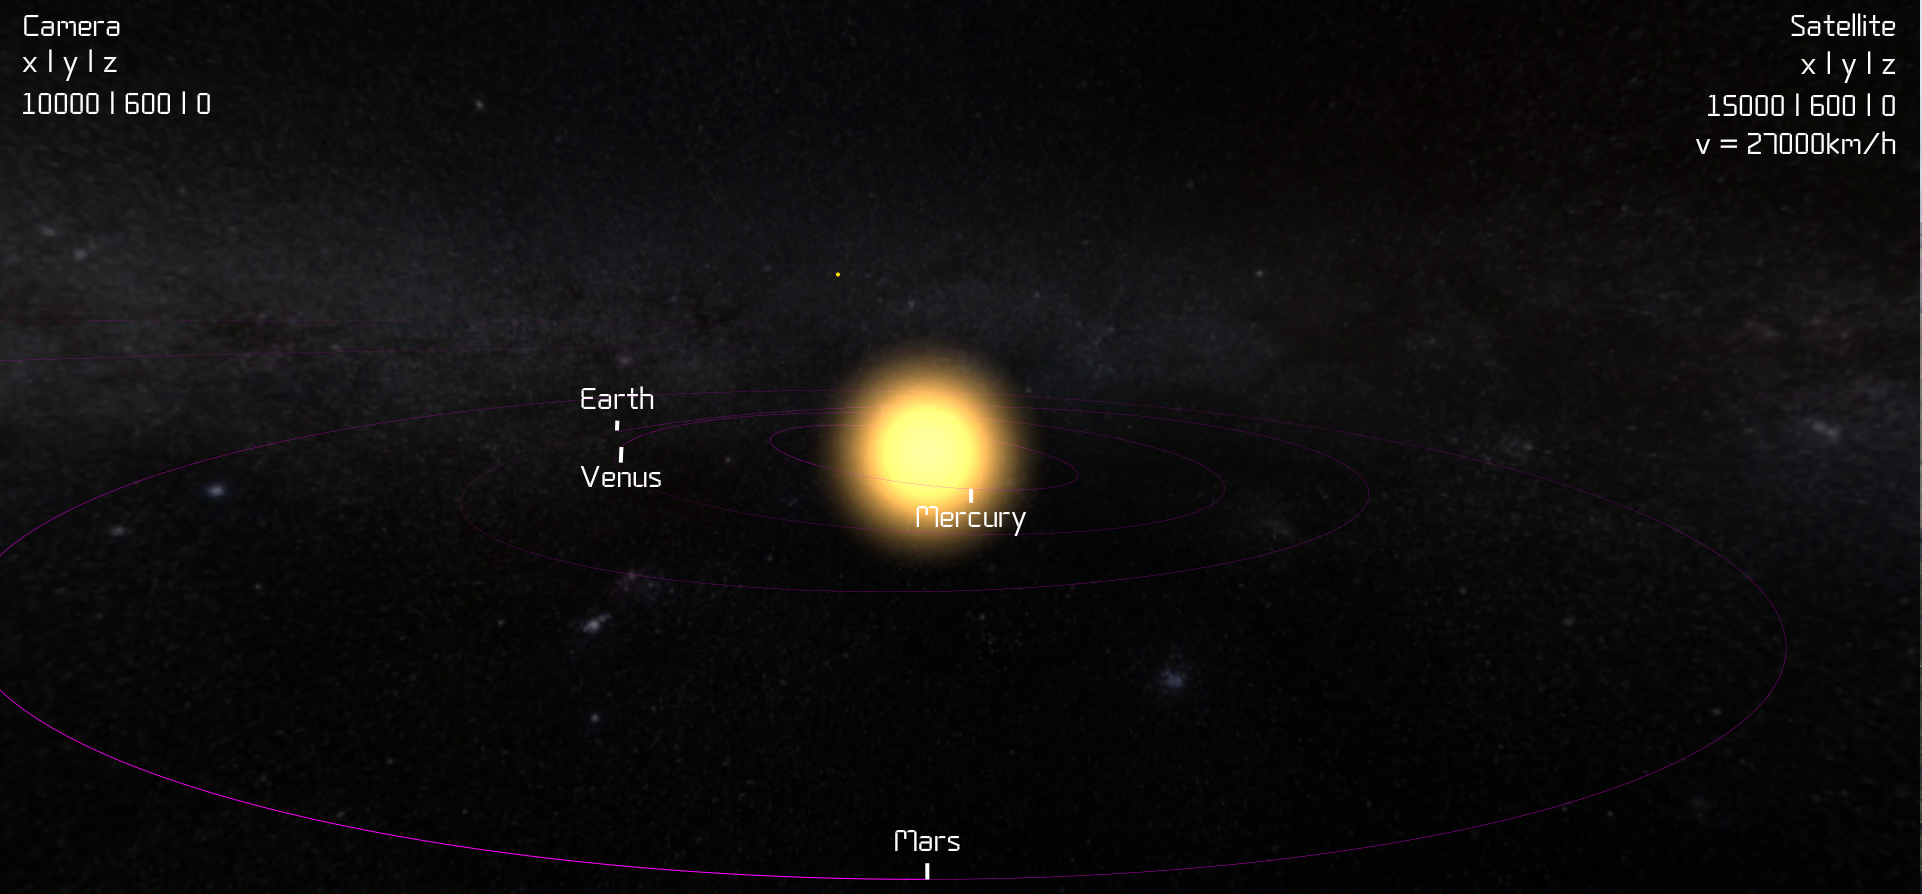
\includegraphics[scale=0.35]{OrbitcalcUI.png}
	\caption{Mockup of the User Interface}
\end{figure}


%\subsection{Source Code}

%\noindent The following environment shows the correct and mandatory way to insert your code.
%\begin{lstlisting}[language=Python, caption=Caption example.]
%import numpy as np
    
%def incmatrix(genl1,genl2):
 %   m = len(genl1)
  %  n = len(genl2)
   % M = None #to become the incidence matrix
   % VT = np.zeros((n*m,1), int)  #dummy variable
    
   % #compute the bitwise xor matrix
   % M1 = bitxormatrix(genl1)
   % M2 = np.triu(bitxormatrix(genl2),1) 

   % for i in range(m-1):
   %     for j in range(i+1, m):
   %         [r,c] = np.where(M2 == M1[i,j])
   %         for k in range(len(r)):
   %             VT[(i)*n + r[k]] = 1;
   %             VT[(i)*n + c[k]] = 1;
   %             VT[(j)*n + r[k]] = 1;
   %             VT[(j)*n + c[k]] = 1;
   %             
   %             if M is None:
   %                 M = np.copy(VT)
   %             else:
   %                 M = np.concatenate((M, VT), 1)
   %             
   %             VT = np.zeros((n*m,1), int)
    
   % return M
%\end{lstlisting}
% that's all folks

\end{document}


